\documentclass[usenames,dvipsnames]{article}

\usepackage{pgf}
\usepackage{tikz}
\usetikzlibrary{arrows,automata}
\usepackage[latin1]{inputenc}
\usepackage{verbatim}
\usepackage{xcolor}
\newcommand{\lightgrey}{black!10}
\newcommand{\darkgrey}{black!40}
\begin{document}
  \pagestyle{empty}
  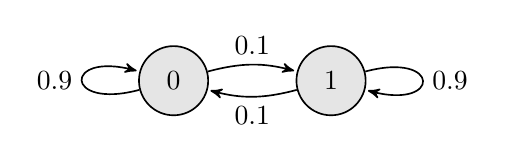
\begin{tikzpicture}[->,>=stealth',shorten >=1pt,auto,node distance=4cm,semithick]
    \tikzstyle{every state}=[fill=\lightgrey,draw=black,text=black]
    \tikzset{every loop/.style={min distance=10mm,looseness=10}}
    \node[state] (0) at (0, 0) {$0$};
    \node[state] (1) at (2, 0) {$1$};
    \path (0) edge [loop left] node {$0.9$} (0);
    \path (0) edge [bend left=15] node {$0.1$} (1);
    \path (1) edge [bend left=15] node {$0.1$} (0);
    \path (1) edge [loop right] node {$0.9$} (1);
  \end{tikzpicture}
\end{document}
